\documentclass{standalone}
\begin{document}
	\chapter{Pipeline}
	
	The aim of these work of thesis is the developing of a automatic pipeline for the segmentation of Ground Galass Opacities and Consolidation areas in chest CT scans of patients affected by COVID-19.
	
	Austin in \textit{Glossary of terms for CT of the lungs}~\cite{ART:Austin} has defined the GGO and CS as : 
	\begin{center}
		"\emph{Hazy increased attenuation of lung, but with preservation of bronchial and vascular margins; caused by partial filling of air spaces, interstitial thickening, partial collapse of alveoli,normal expiration, or increased capillary blood volume, which is different from consolidation in which bronchovascular margins are obscured.}
	\end{center}. 

	\begin{figure}[ht]
		\begin{subfigure}{.5\textwidth}
			\centering
			% include first image
			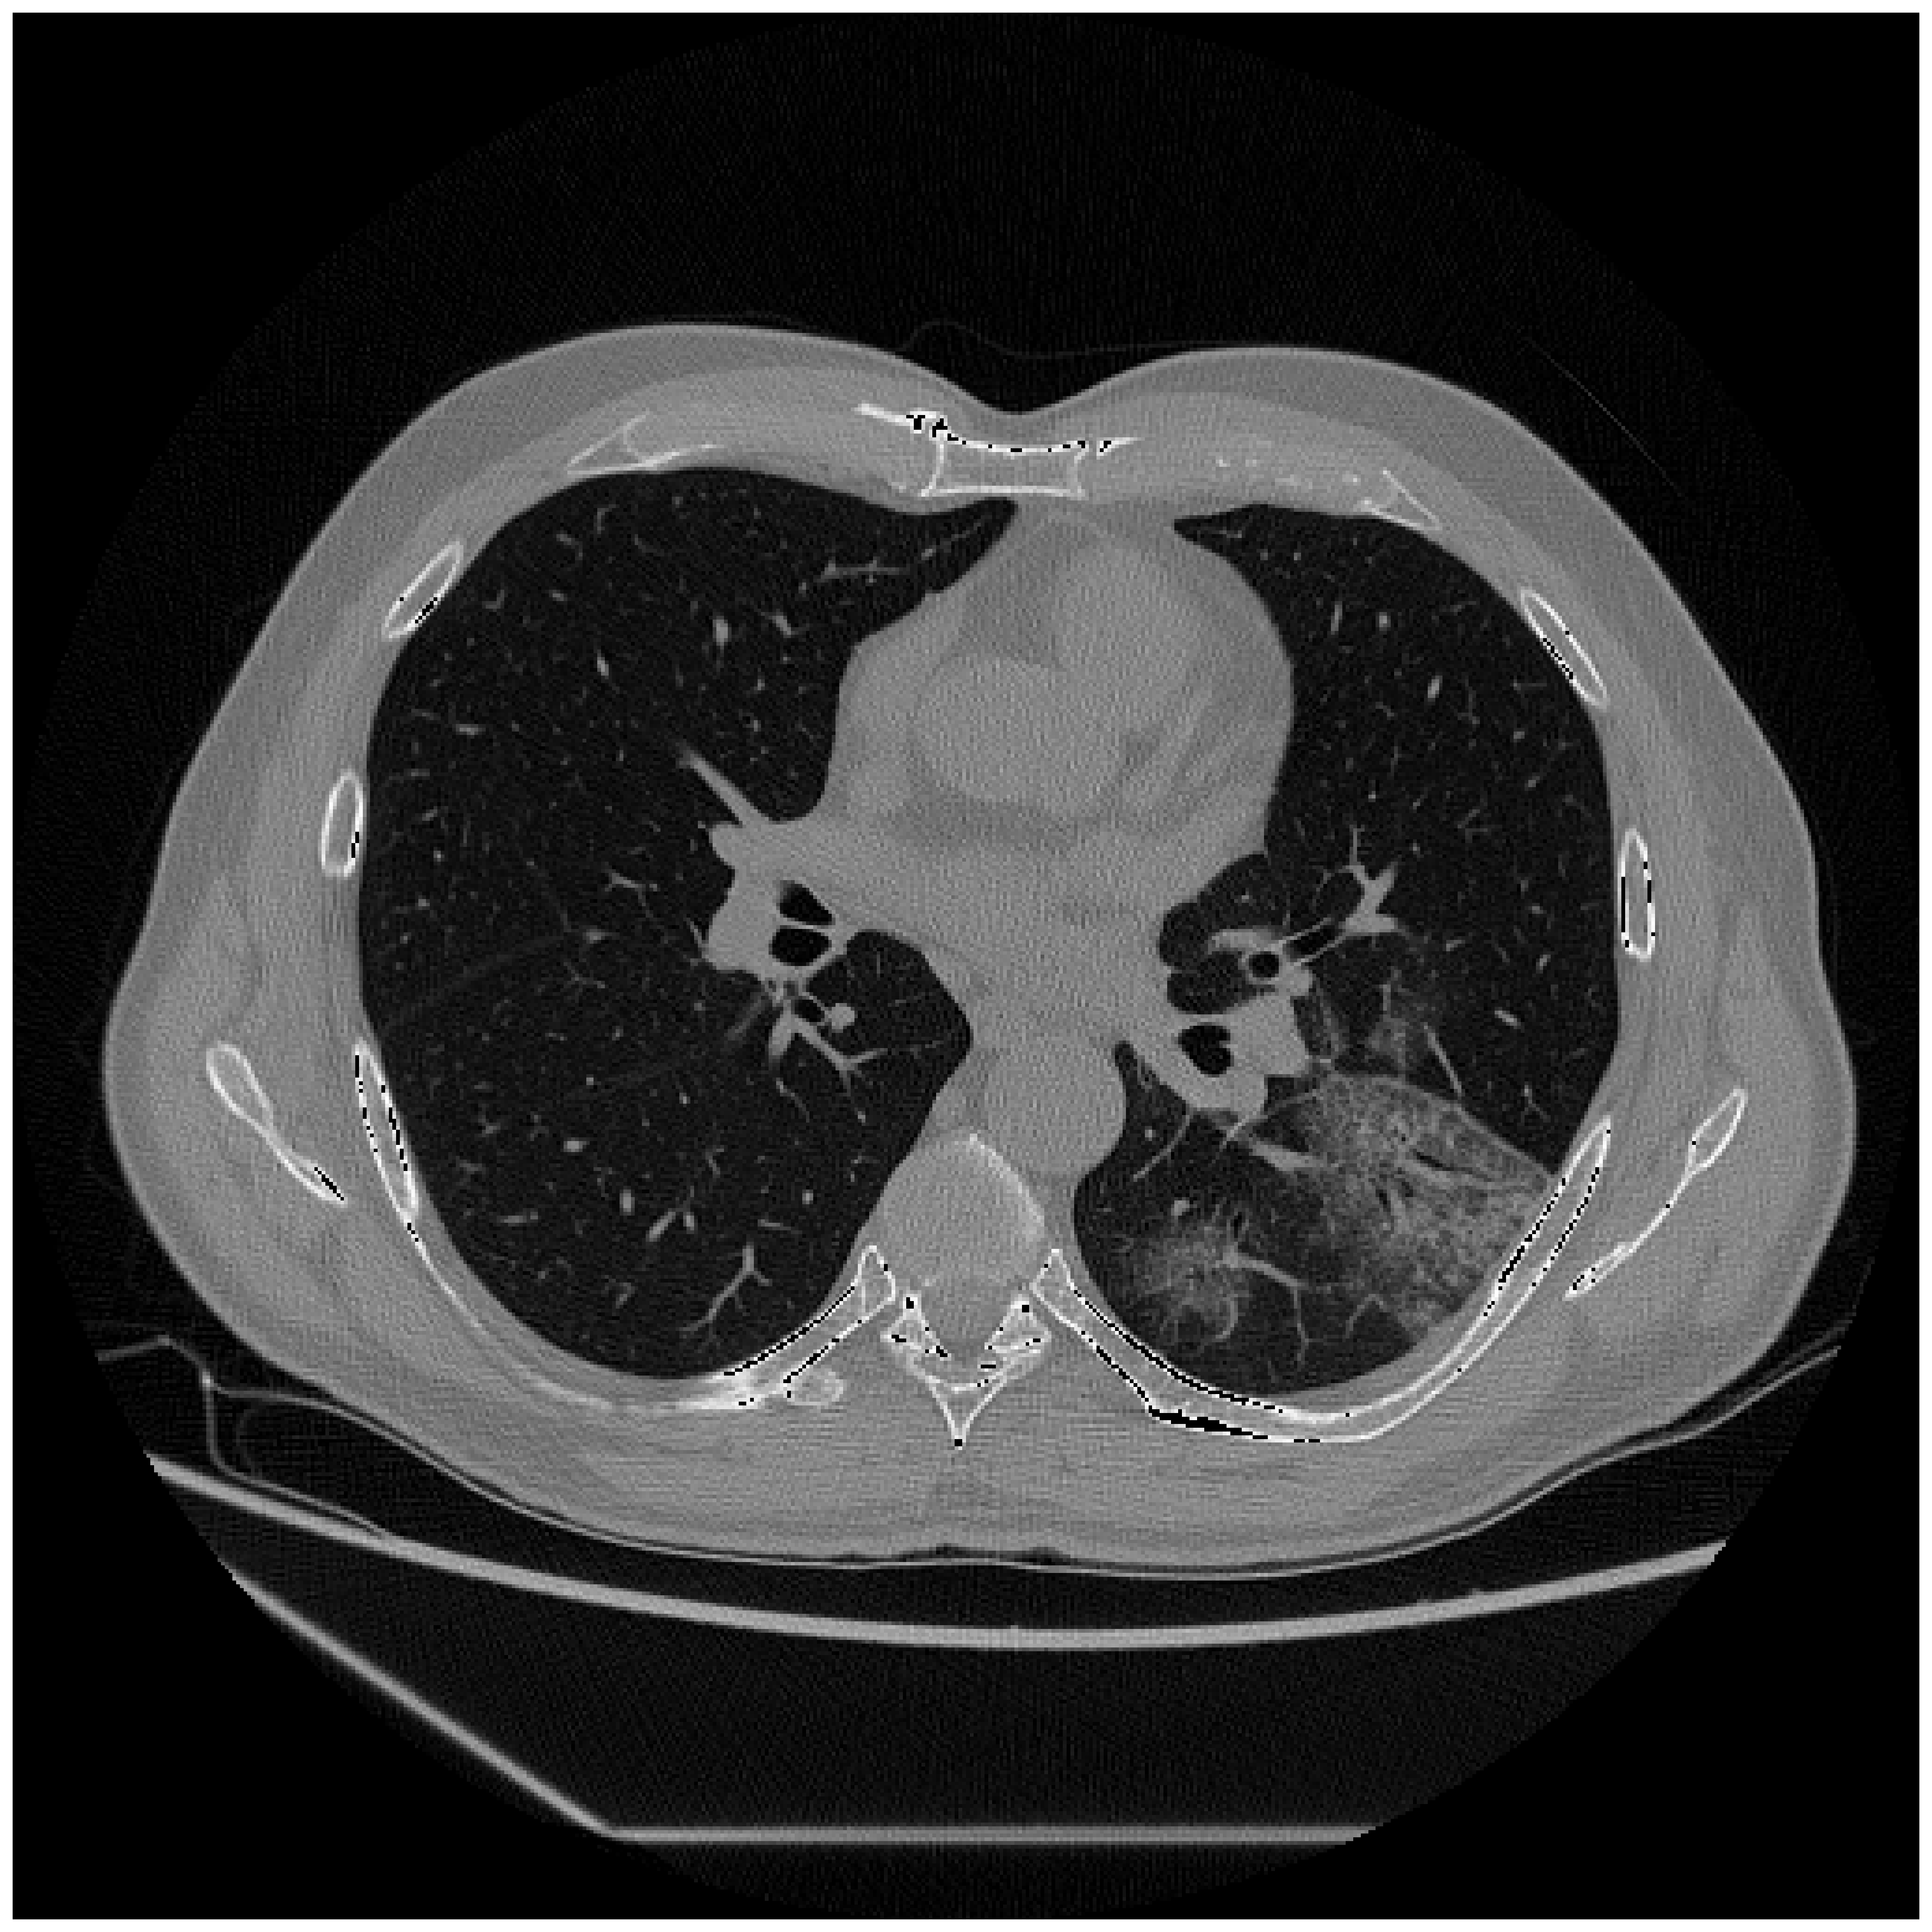
\includegraphics[width=.8\linewidth]{CVscan.png}  
			\caption{Chest CT scan of a patient affected by COVID-19}
			\label{fig:CTscan}
		\end{subfigure}
		\begin{subfigure}{.5\textwidth}
			\centering
			% include second image
			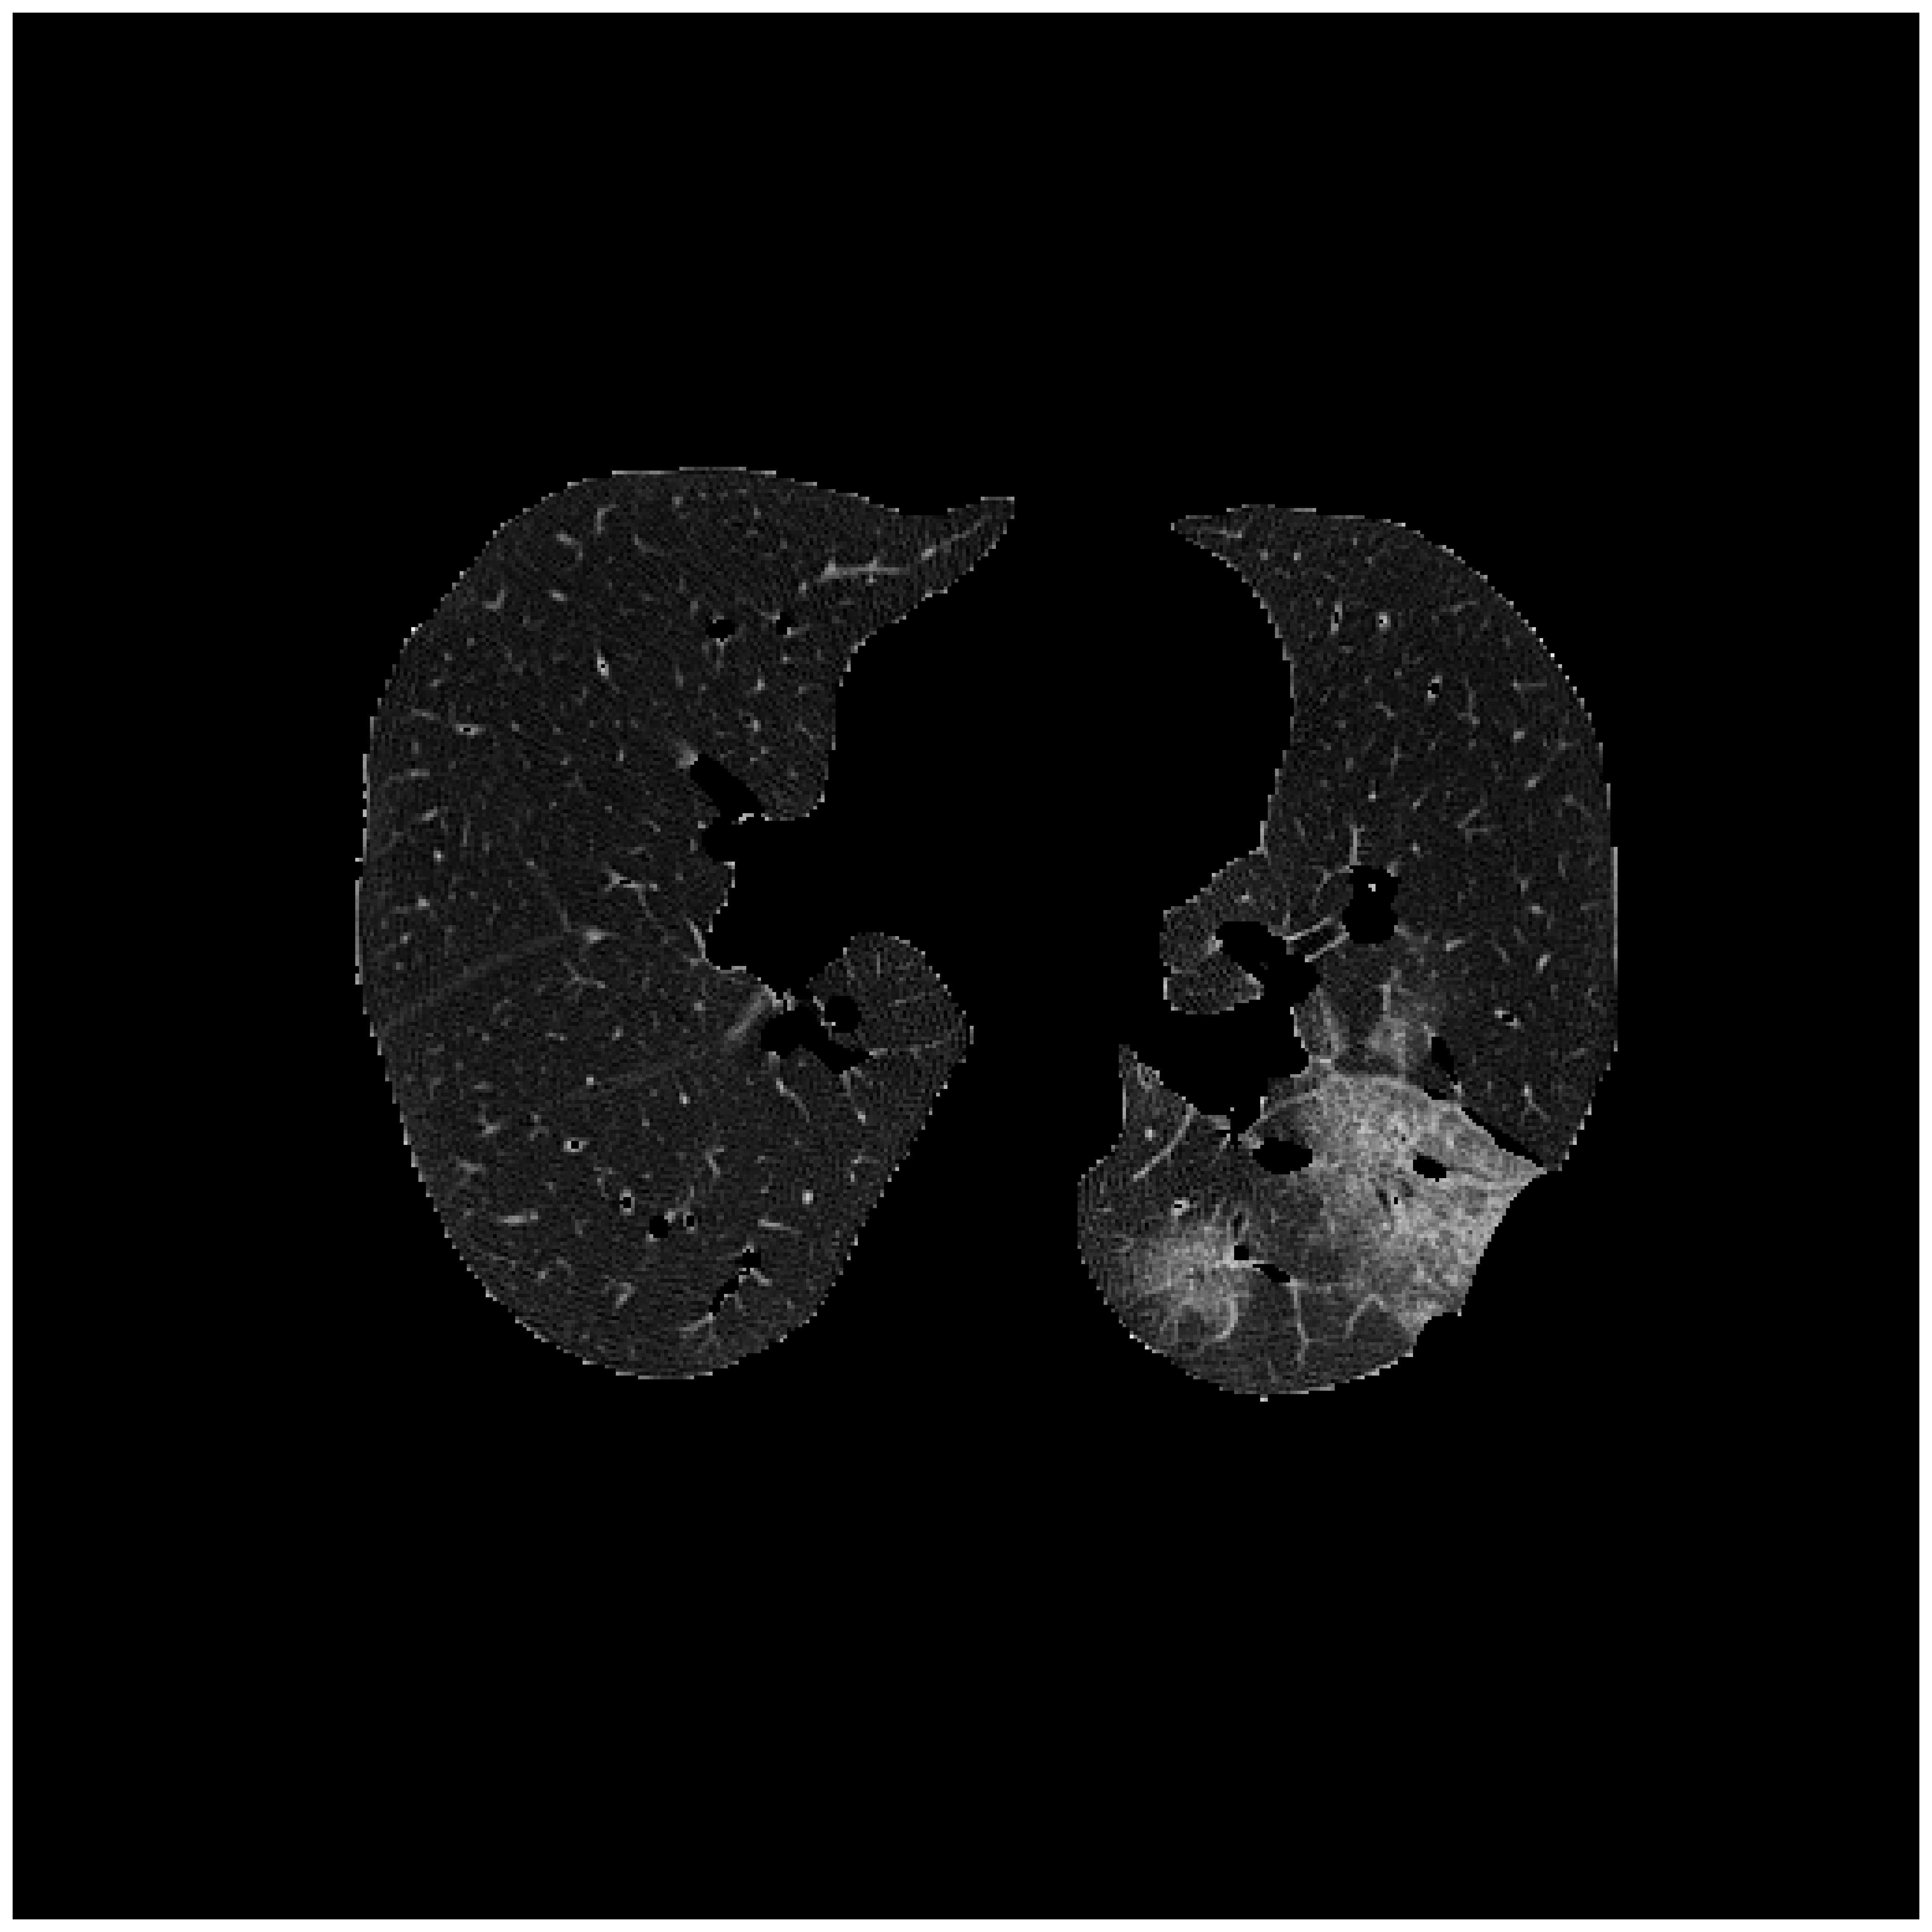
\includegraphics[width=.8\linewidth]{Lung_Extracted.png}  
			\caption{Isolated lung regions}
			\label{fig:lung}
		\end{subfigure}
		\caption{Original Chest CT scan(a), we can clearly see the GGO and CS regions. Moreover all extra -lung regions are present. In (b) we can see the same slice but after the lung segmentation. We can see that each different region has a similar gray level.}
		\label{fig:CTLung}
	\end{figure}


	The starting point are the chest CT scans (\figurename\,\ref{fig:CTscan}). Firstly I have removed all the extra lung regions like body, bronchial structures and CT tube which are a potential source of false positives. Once we have obtained a scan as \figurename\,\ref{fig:lung}, we can notice that  the different structures are characterized by similar gray level: the basic idea was to use the color quantization for medical image segmentation, grouping voxels based on color similarity, and  assigning  to each tissue a characteristic color. This can be done since in CT scan exists a relationship between the tissue in the voxels and the Gray Levels used to display it, given by the Hounsfiend Units(eq\,\ref{eq:HU}): the colors are proportional to HU, which are defined as a linear transformation of the linear attenuation coefficient($\mu$).
	
	We can consider different properties beside the single voxel intensity. As we can see, lesion areas involves many closest voxels. It is interesting to incorporates also neighborhood voxel information in the color quantization. Moreover, contrast between sick and healthy areas may change according to the severity of the disease. As a consequence it is interesting to incorporates also different gamma of the image, in order to enhance these regions.
	
	Digital images may have more than one \textit{sample per pixel}. For a color image each voxel is represented by 3 sample, one for each primary color. I can use color to encode also more informations, exploited with the application of different functions in the image. In this way I've build a color space which encode different image features.
	
	Once I have build the color space, I have to find the characteristic color of each tissue under study, which is represented by a centroids in the color space. I have created a training dataset made of CT scans from different patients and applied a  k-means clustering, since it provides a good balance between segmentation performance and computational efficiency. K-means clustering requires a prior knowledge about the number of cluster, which in our case is given by the anatomical structure of the lung. I have consider a different cluster for each anatomical structure : 
		\begin{itemize}
		\item Lung Parenchima; 
		
		\item  Edges;
		
		\item Vessel surrounding bronchial structures;
		
		\item Bronchi.
		
		\item  Ground Glass Opacities and consolidation;
		
	\end{itemize}
		
	Once I have estimated the centroids for each tissue, I have used them for the  segmentation: each voxel of the image  is assigned  to the cluster of the closest centroids.
	
	The final pipeline structure is summarized in \figurename\,\ref{Pipeline}.
	
	\begin{figure}[h!]
		\centering
		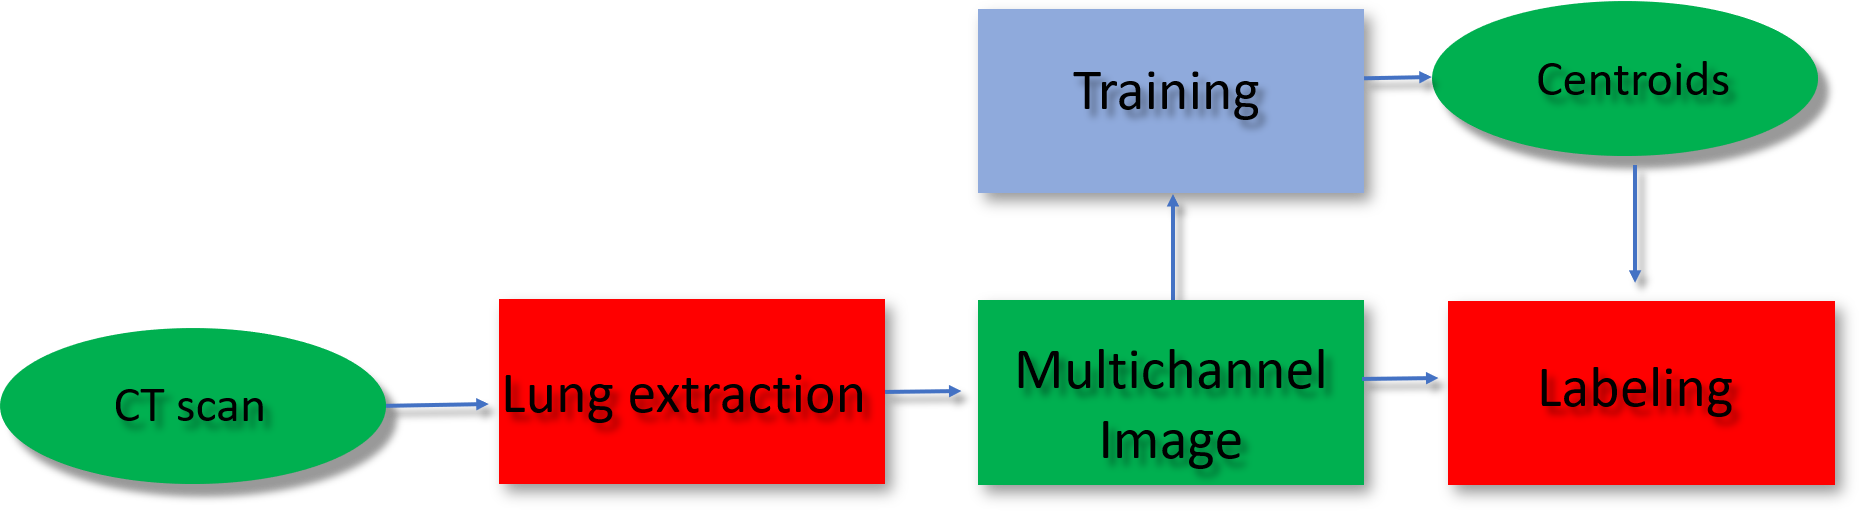
\includegraphics[width=.87\textwidth]{Pipeline.png}
		\caption{Actual segmentation step, from left to right we can see the input image stack, the isolated lung regions and the final label. To performed the labeling a set of pre-computed centroids was used.}\label{fig:Pipeline}
	\end{figure}


	Once the centroids are estimated, the training step does not nedds to be repeated. Moreover, in the implementation, the building of the multichannel image is incorporated in the labeling step. As a consequence the final pipline structure looks like in \figurename\,\ref{fig:FinalPipeline}.
	
	\begin{figure}[h!]
		\centering
		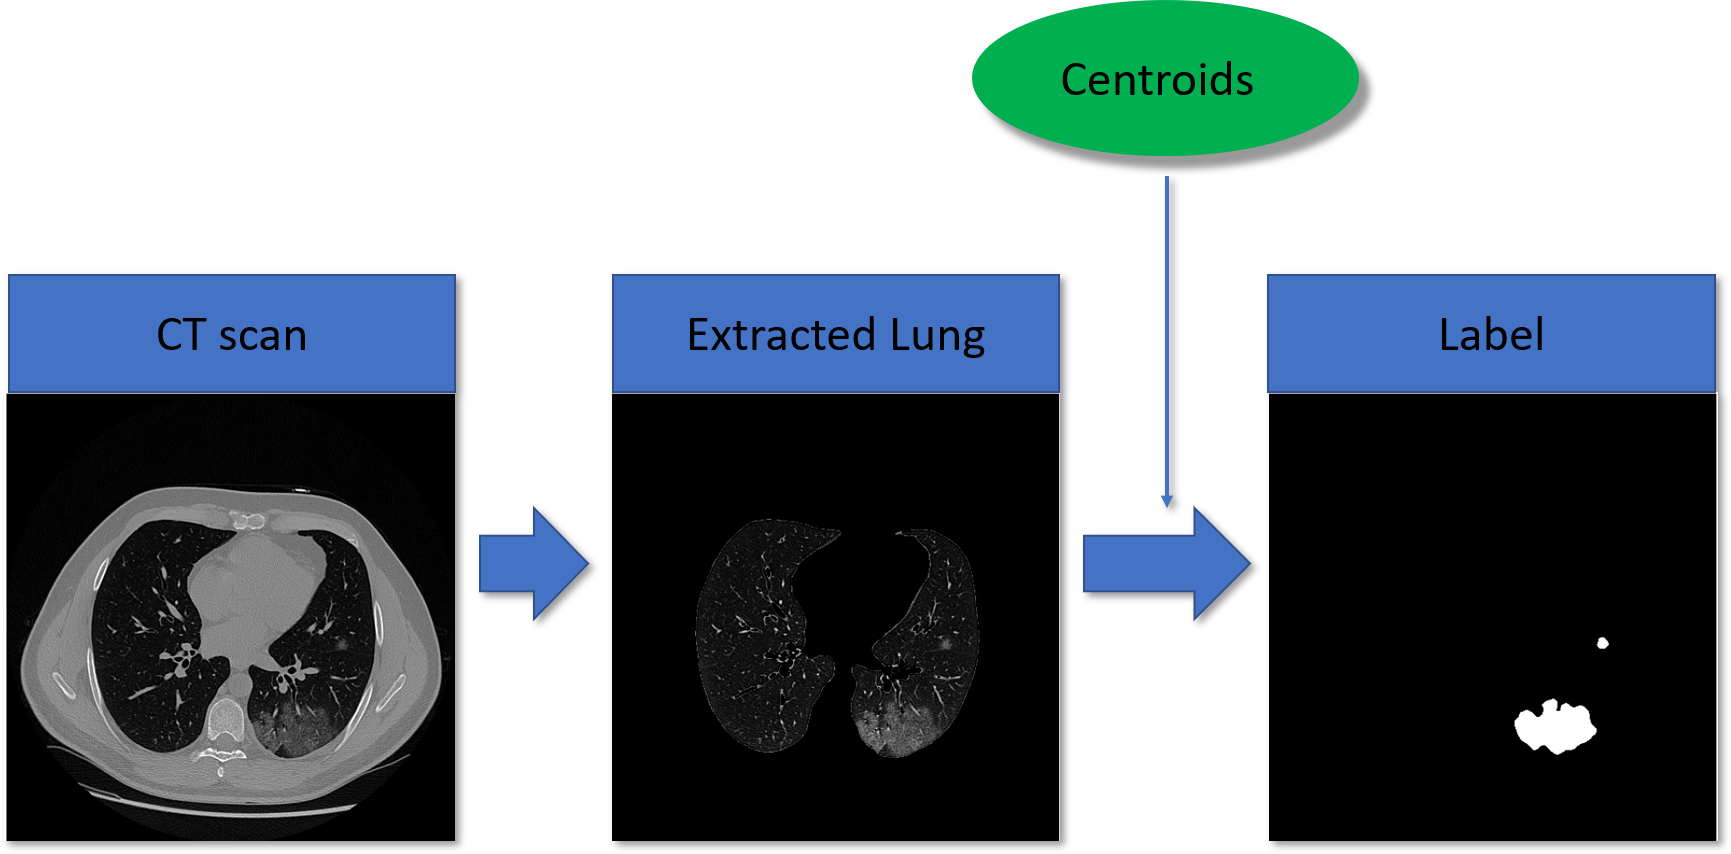
\includegraphics[width=.87\textwidth]{final_pipeline.png}
		\caption{Actual segmentation step, from left to right we can see the input image stack, the isolated lung regions and the final label. To performed the labeling a set of pre-computed centroids was used.}\label{fig:FinalPipeline}
	\end{figure}
	
	
	
	
	
	
	
	
\end{document}